\chapter{Questionnaire 2: User Study of Utsida}
\label{app:questionnaire2}

\section{Predefined Queries}
\label{appendix:pre_defined_search}

\begin{table}[h]
\centering
\caption[]{Predefined search queries used in questionnaire 2}
\label{pre_defined_search_table}
\begin{tabular}{|l|l|l|}
\hline
\textbf{Query}               & \textbf{Query 1}             & \textbf{Query 2}                                                                              \\ \hline
\textbf{Institute}           & Institutt for elkraftteknikk & \begin{tabular}[c]{@{}l@{}}Institutt for datateknikk og\\  informasjonsvitenskap\end{tabular} \\ \hline
\textbf{Continent}           & North America                & Europe                                                                                        \\ \hline
\textbf{Country}             & USA                          & Frankrike                                                                                     \\ \hline
\textbf{University}          &                              &                                                                                               \\ \hline
\textbf{Language}            & Engelsk                      & Fransk                                                                                        \\ \hline
\textbf{Study Period}        & 2017                         & 2017                                                                                          \\ \hline
\textbf{Academic Quality}    & 6                            & 8                                                                                             \\ \hline
\textbf{Social Quality}      & 9                            & 4                                                                                             \\ \hline
\textbf{Residential Quality} & 7                            & 6                                                                                             \\ \hline
\textbf{Reception Quality}   & 3                            & 3                                                                                             \\ \hline
\end{tabular}
\end{table}


\FloatBarrier
\section{Open Question Results} \label{app:questionnaire2_open_question}

\begin{table}[H]
\centering
\caption[]{Theme Analysis}
\label{app:tab:open_questionnaire2}
\resizebox{\textwidth}{!}{%
\begin{tabular}{|l|l|l|l|l|l|l|l|l|l|l|l|l|l|l|l|l|l|l|l|l|l|}
\hline
\rowcolor[HTML]{C0C0C0} 
Category & \#1 & 2 & 3 & 4 & 5 & 6 & 7 & 8 & 9 & 10 & 11 & 12 & 13 & 14 & 15 & 16 & 17 & 18 & 19 & 20 & SUM \\ \hline
Positive feedback & * & * &  &  &  & * &  & * & * &  &  &  & * & * &  &  & * & * & * & * & 11 \\ \hline
non-intuitive &  &  &  & * &  &  & * &  &  & * &  &  &  & * & * &  &  &  &  &  & 5 \\ \hline
Easy to use &  & * &  &  & * &  &  &  &  &  &  & * &  &  & * &  &  &  &  &  & 4 \\ \hline
Time saving & * &  &  &  &  &  &  &  &  &  &  &  &  &  &  &  &  &  & * & * & 3 \\ \hline
\begin{tabular}[c]{@{}l@{}}Great use of \\ experience reports\end{tabular} &  &  &  &  & * &  &  &  &  &  &  &  &  &  & * &  &  &  &  &  & 2 \\ \hline
Good recommendations & * &  &  &  &  &  &  &  &  &  &  &  &  &  &  &  &  &  &  &  & 1 \\ \hline
\begin{tabular}[c]{@{}l@{}}Does not fit \\ well for mixed studies\end{tabular} &  &  &  &  &  &  & * &  &  &  &  &  &  &  &  &  &  &  &  &  & 1 \\ \hline
Great to be self-serviced &  &  &  &  &  &  &  &  &  &  &  &  &  &  &  &  &  &  & * &  & 1 \\ \hline
Idividual adaption &  &  &  &  &  &  &  &  &  &  &  &  &  &  &  &  &  &  &  & * & 1 \\ \hline
\end{tabular}
}
\end{table}



\FloatBarrier
\section{Questions}\label{app:questionnaire2_questions}

\begin{figure}[h]
    \centering
    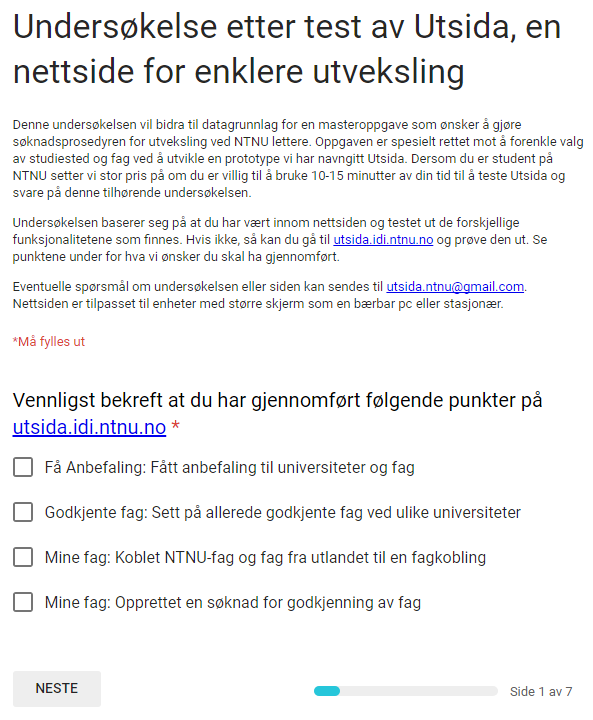
\includegraphics[width=0.8\textwidth]{fig/form2/front.PNG}
    \caption[]{The introduction to the questionnaire}
    \label{fig:questionnaire_2_questions_p1}
\end{figure}
\begin{figure}[h]
    \centering
    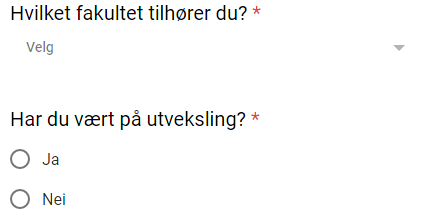
\includegraphics[width=0.6\textwidth]{fig/form2/s2.PNG}
    \caption[]{Question 1: Demographics}
    \label{fig:questionnaire_2_questions_p2}
\end{figure}
\begin{figure}[h]
    \centering
    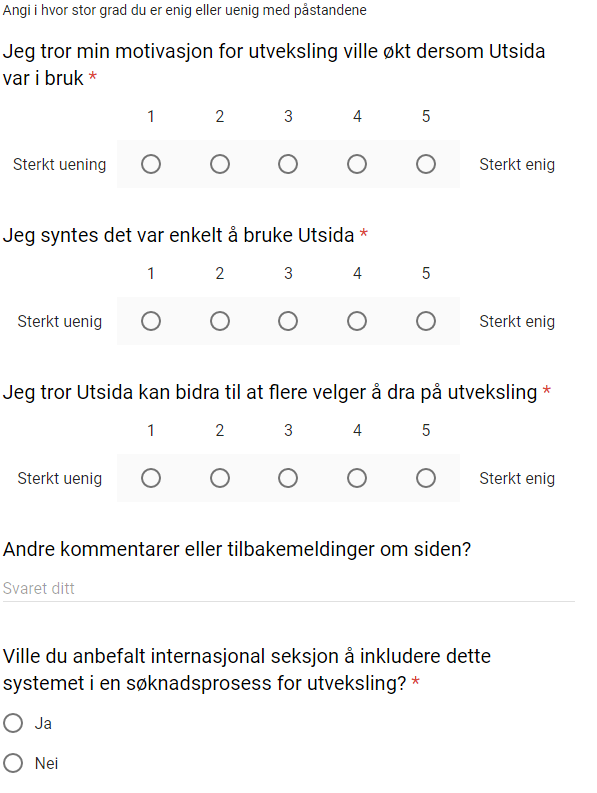
\includegraphics[width=1\textwidth]{fig/form2/s3.PNG}
    \caption[]{Questions regarding motivational effect on students who have not been on exchange}
    \label{fig:questionnaire_2_questions_p3}
\end{figure}
\begin{figure}[h]
    \centering
    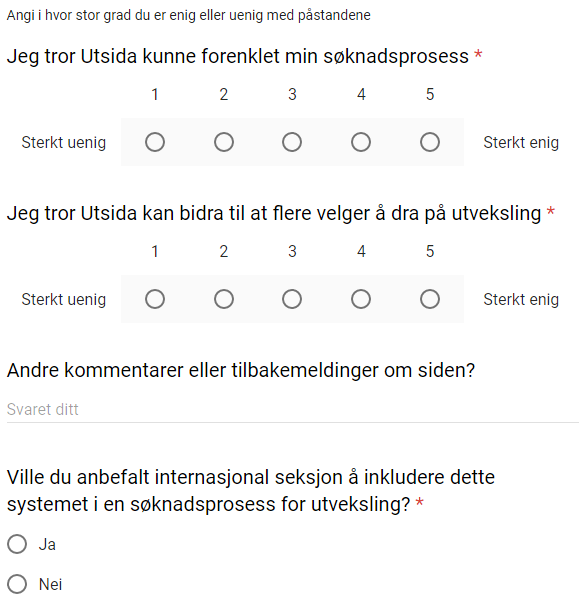
\includegraphics[width=1\textwidth]{fig/form2/s4.PNG}
    \caption[]{Questions regarding motivational effect on students who have already been on exchange}
    \label{fig:questionnaire_2_questions_p4}
\end{figure}
\begin{figure}[h]
    \centering
    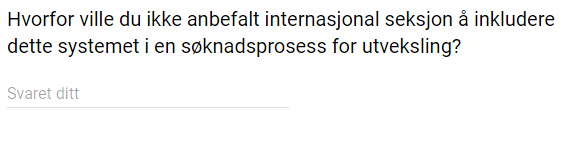
\includegraphics[width=1\textwidth]{fig/form2/s5.PNG}
    \caption[]{Question given to participants who answered \enquote{No} on the past quetion}
    \label{fig:questionnaire_2_questions_p5}
\end{figure}
\begin{figure}[h]
    \centering
    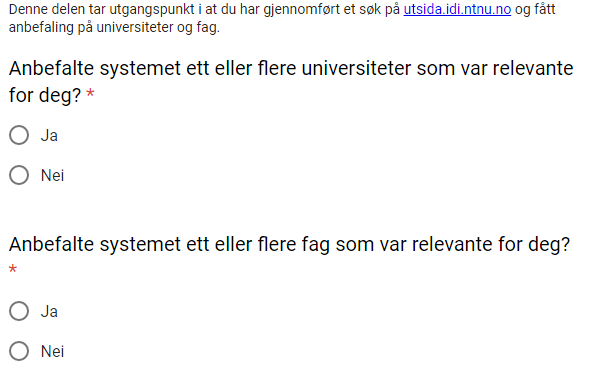
\includegraphics[width=1\textwidth]{fig/form2/s6.PNG}
    \caption[]{Question asking about the recommendations the participants received during the test}
    \label{fig:questionnaire_2_questions_p6}
\end{figure}
\begin{figure}[h]
    \centering
    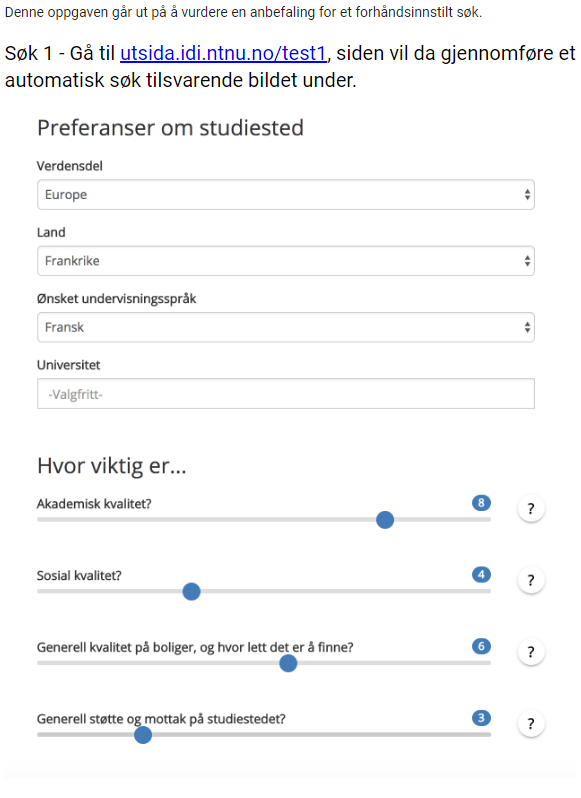
\includegraphics[width=1\textwidth]{fig/form2/s7_1.PNG}
    \caption[]{The first predesigned query}
    \label{fig:questionnaire_2_questions_p7}
\end{figure}
\begin{figure}[h]
    \centering
    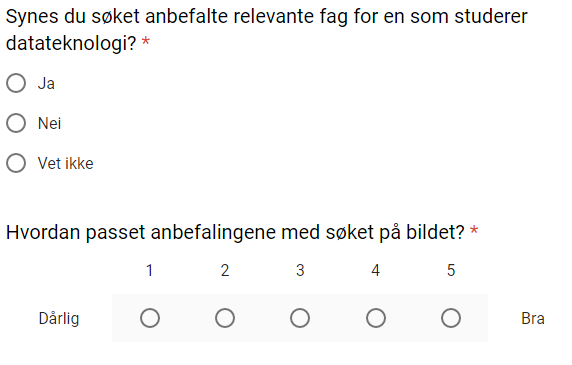
\includegraphics[width=1\textwidth]{fig/form2/s7_2.PNG}
    \caption[]{Evaulation of the first predesigned query}
    \label{fig:questionnaire_2_questions_p8}
\end{figure}
\begin{figure}[h]
    \centering
    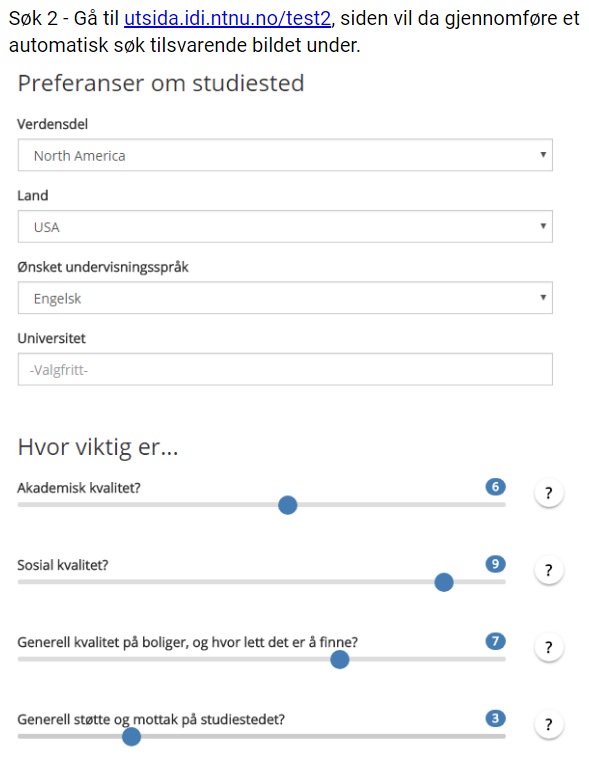
\includegraphics[width=1\textwidth]{fig/form2/s7_3.PNG}
    \caption[]{Second predesigned query}
    \label{fig:questionnaire_2_questions_p9}
\end{figure}
\begin{figure}[h]
    \centering
    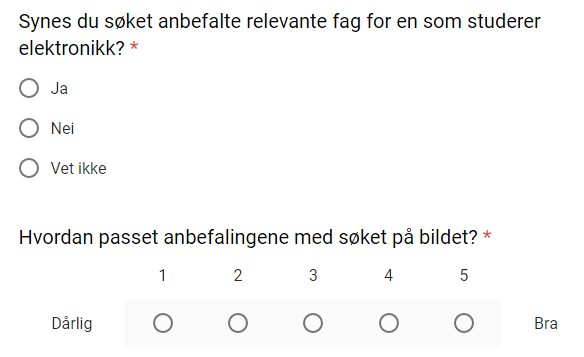
\includegraphics[width=1\textwidth]{fig/form2/s7_4.PNG}
    \caption[]{Evaulation of the second predesigned query}
    \label{fig:questionnaire_2_questions_p10}
\end{figure}